\section{Box-counting dimenze}\label{sec:box-counting-dimenze}

Tomuto typu dimenze jsme se již v~základu věnovali v~kapitole \ref{chapter:uvod_do_fraktalu},~specificky sekci \ref{sec:fraktalni_dimenze},~kde jsme rozebrali jeho způsob jejího výpočtu a ukázali jsme si jej několika příkladech. V~této části si blíže rozebereme některé další vlastnosti týkající se právě \emph{box-counting dimenze}\index{box-counting dimenze}\footnote{V kapitole \ref{chapter:uvod_do_fraktalu} jsme pro jednoduchost používali obecnější termín \emph{fraktální dimenze}. Ten však zahrnuje daleko širší škálu možných definic,~než jen tu,~kterou jsme si představili. Avšak dále v~tomto textu budeme používat výhradně její skutečný název,~tj. box-counting dimenze.} a pokusíme se ji lépe zasadit do kontextu teorie míry,~které jsme se samostatně až do této chvíle věnovali.

\subsection{Definice a výpočet}\label{subsec:definice-a-vypocet-bc-dimenze}

Jako první se podíváme na myšlenku box-counting trochu blíže a maličko si ji zobecníme. Původně jsme nahlíželi na dimenzi jako na exponent,~s nímž roste "velikost" zkoumaného útvaru. Tato myšlenka nás se ukázala jako rozumná,~neboť pro "klasické" geometrické útvary vycházela tato dimenze vždy celočíselně,~nicméně už tomu tak nebylo v~případě fraktálních útvarů. Myšlenka byla taková,~že jsme útvar $F$ rozdělili na určitý počet stejně "velkých částí",~označme $F_1,F_2,\ldots,F_m$,~v nějakém měřítku $\varepsilon>0$. Zkusme nyní požadavek na striktně stejnou velikost (formálně vzato míru) trochu rozvolnit. Bude nám stačit,~když pro každé $i$ je $\diam{F_i}\leqslant\delta$,~kde $\delta>0$. Zároveň nebudeme požadovat,~aby množiny\linebreak{}$F_1,F_2,\ldots,F_m$ byly všechny striktně po dvou téměř disjunktními\footnote{Množiny $M,N$ jsou \emph{téměř disjunktní},~pokud $\interior{M}\cap\interior{N}=\emptyset$,~tedy může nastat,~že se na hranici mohou "dotýkat",~tzn. $\boundary{M}\cap\boundary{N}\neq\emptyset$.} podmnožinami $F$,~ale stačí,~když budou tvořit pokrytí $F$.

Mějme tedy nějakou neprázdnoou omezenou množinu $F\subset\R^n$,~kde pro každé $\delta>0$ budeme hledat \emph{nejmenší počet} množin,~takových,~že pokrývají $F$. Toto číslo si označíme $N_\delta(F)$. Dimenze množiny $F$ by tedy měla odrážet "rychlost" růstu $N_\delta(F)$ pro $\delta\to 0^+$. Je-li splněna aproximace
\begin{equation}\label{eq:odhad-n-delta}
    N_\delta(F)\approx c\delta^{-s}
\end{equation}
pro $c>0$,~pak řekneme,~že množina $F$ má box-counting dimenzi $s$. (Převzato z~\citep[str. 27]{Falconer2014}.)
\begin{remark}
    V~dalším textu budeme místo $\delta\to 0^+$ psát pro jednoduchost pouze $\delta\to 0$,~byť by se slušilo používat první variantu. Čtenáři je však nejspíše jasné,~že uvažovat záporný průměr množiny nemá smysl.
\end{remark}
Logaritmováním a úpravou výrazu \eqref{eq:odhad-n-delta} dostaneme:
\begin{align}\label{eq:odvozeni-box-counting-dimenze}
    \ln{N_\delta(F)}&\approx\ln{c}+\ln{\delta^{-s}}\\
    \ln{N_\delta(F)}&\approx\ln{c}-s\ln{\delta}\\
    s&\approx\dfrac{\ln{N_\delta(F)}}{-\ln{\delta}}+\dfrac{\ln{c}}{\ln{\delta}}.
\end{align}
Když porovnáme výsledek v~\eqref{eq:odvozeni-box-counting-dimenze} s~rovností \eqref{eq:fraktalni-dimenze} z~minulé kapitoly,~můžeme si všimnout,~že zde navíc figuruje člen $\ln{c}/\ln{\delta}$. Když však uvážíme limitu daného výrazu pro $\delta\to 0$,~dostaneme původní vzorec,~který jsme již viděli,~tj.
\[\lim_{\delta\to 0}\left(\dfrac{\ln{N_\delta(F)}}{-\ln{\delta}}+\dfrac{\ln{c}}{\ln{\delta}}\right)=\lim_{\delta\to 0}\dfrac{\ln{N_\delta(F)}}{-\ln{\delta}}+\lim_{\delta\to 0}\dfrac{\ln{c}}{\ln{\delta}}=\lim_{\delta\to 0}\dfrac{\ln{N_\delta(F)}}{-\ln{\delta}}.\]
% \begin{definition}[$\delta$-pokrytí]\label{def:delta-pokryti}
%     Nechť $(X,\rho)$ je metrický prostor,~$F\subseteq X$ a $\delta>0$. Jestliže $\mathcal{F}=\set{F_1,F_2,\ldots}\subseteq\powset{X}$ je pokrytí $F$ a zároveň $\diam{F_j}\leqslant\delta$ pro každé $j$,~pak $\mathcal{F}$ nazýváme $\delta$-pokrytí\index{$\delta$-pokrytí} množiny $F$.
% \end{definition}
Předchozí úvahu můžeme shrnout do následující definice.
\begin{definition}[Box-counting dimenze]\label{def:box-counting-dimenze}
    Nechť $F\subset \R^n$ je neprázdná omezená množina. Pak definujeme následující:
    \begin{enumerate}[label=(\alph*)]
        \item \emph{Nejmenší počet množin v~$\delta$-pokrytí množiny $F$} značíme $N_\delta(F)$,~tj.
        \[N_\delta(F)=\inf\set{m\in\N_0\;\middle|\;F\subseteq\bigcup_{i=1}^n F_i\;,\;\diam{F_j}\leqslant\delta\;\text{pro}\;1\leqslant j\leqslant m}.\]
        \item \emph{Horní box-counting dimenze}\index{box-counting dimenze!horní box-counting dimenze} množiny $F$ je
        \[\upperdimB{F}=\limsup_{\delta\to 0}\dfrac{\ln{N_\delta(F)}}{-\ln{\delta}}.\]
        \item \emph{Dolní box-counting dimenze}\index{box-counting dimenze!dolní box-counting dimenze} množiny $F$ je
        \[\lowerdimB{F}=\liminf_{\delta\to 0}\dfrac{\ln{N_\delta(F)}}{-\ln{\delta}}.\]
    \end{enumerate}
    V~případě,~že $\lowerdimB{F}=\upperdimB{F}$,~pak společnou hodnotu nazýváme \emph{box-counting dimenzí}\index{box-counting dimenze} množiny $F$,~značíme $\dimB{F}$,~přičemž platí
    \[\dimB{F}=\lim_{\delta\to 0}\dfrac{\ln{N_\delta(F)}}{-\ln{\delta}}.\]
\end{definition}
\begin{remark}
    Zde je důležité zmínit,~že pro v~dalším textu budeme uvažovat $\delta$ dostatečně malé,~takové,~že hodnota $-\ln{\delta}$ je vždy kladná. Dále též budeme pracovat (podle definice \ref{def:box-counting-dimenze}) pouze s~neprázdnými omezenými množinami,~abychom se vyhnuli problémům s~případy,~kdy $N_\delta(F)=\infty$ nebo $N_\delta(F)=0$.
\end{remark}
Abychom uvedli vše na pravou míru,~box-counting dimenzi lze taktéž definovat více způsoby. V~tuto uvažujeme obecně $\delta$-pokrytí dané množiny $F$,~tj. pokrytí \emph{obecnými} množinami o~průměru maximálně $\delta>0$. Lze se však zaměřit i~na konkrétní útvary,~jak ukazuje následující věta.
\begin{theorem}[Ekvivalentní definice box-counting dimenze]\label{thm:ekvivalentni-def-box-counting-dimenze}
    Nechť $F\subset \R^n$ je neprázdná omezená množina. Pak
    \begin{align*}
        \lowerdimB{F}&=\liminf_{\delta\to 0}\dfrac{\ln{M_\delta(F)}}{-\ln{\delta}},\\
        \upperdimB{F}&=\limsup_{\delta\to 0}\dfrac{\ln{M_\delta(F)}}{-\ln{\delta}},\\
        \dimB{F}&=\lim_{\delta\to 0}\dfrac{\ln{M_\delta(F)}}{-\ln{\delta}},
    \end{align*}
    kde pro $M_\delta(F)$ platí
    \begin{enumerate}[label=(\roman*)]
        \item\label{thm:pokryti-delta-uz-koulemi} $\displaystyle M_\delta(F)=\inf\set{m\;\middle|\;F\subseteq\bigcup\limits_{i=1}^m K_\delta(x_i)\;,\;x_j\in\R^n\;\text{pro}\;1\leqslant j\leqslant m}$,
        \item\label{thm:pokryti-delta-kvadry} $\displaystyle M_\delta(F)=\inf\set{m\;\middle|\;F\subseteq\bigcup\limits_{i=1}^m I_i\;,\;I_j=\prod_{k=1}^{n}\langle a_k,a_k+\delta\rangle\;\text{pro}\;1\leqslant j\leqslant m}$,
        \item\label{thm:pokryti-delta-sit} $\displaystyle M_\delta(F)=\left|\set{I\;\middle|\;I\cap F\neq\emptyset\;,\;I\in\mathcal{D}}\right|$,~kde $\mathcal{D}$ je $\delta$-síť.
        \item\label{thm:pokryti-delta-dis-ot-koulemi} $\displaystyle M_\delta(F)=\sup\set{m\;\middle|\;B_\delta(x_i)\cap B_\delta(x_j)=\emptyset\;;\;x_i,x_j\in\R^n\;\text{pro}\;1\leqslant i,j\leqslant m}$.
    \end{enumerate}
\end{theorem}

Pojďme si větu \ref{thm:ekvivalentni-def-box-counting-dimenze} nyní trochu rozebrat.
\begin{itemize}
    \item Body \ref{thm:pokryti-delta-uz-koulemi} a \ref{thm:pokryti-delta-dis-ot-koulemi} říkájí,~že $N_\delta(F)$ je rovno \emph{nejmenšímu počtu uzavřených koulí o~poloměru $\delta$,~které pokrývají $F$},~resp. \emph{nejvyšší počet disjunktních otevřených koulí,~které mají střed v~$F$}.
    \item Podobně body \ref{thm:pokryti-delta-kvadry} a \ref{thm:pokryti-delta-sit} tvrdí,~že $N_\delta(F)$ lze ekvivalentně definovat jako pokrytí kvádry o~stranách délky $\delta$,~resp. počet všech kvádrů z~$\delta$-sítě,~které mají s~$F$ neprázdný průnik.
\end{itemize}
Pro představu viz obrázek \ref{fig:ilustrace-definic-bc-dimenze}. Důkaz věty je delší a opět jej vynecháme,~nicméně lze jej nalézt v~knize \citep[str. 30]{Falconer2014}.
\begin{figure}[h]
    \centering
    \begin{subfigure}{0.4\textwidth}
        \centering
        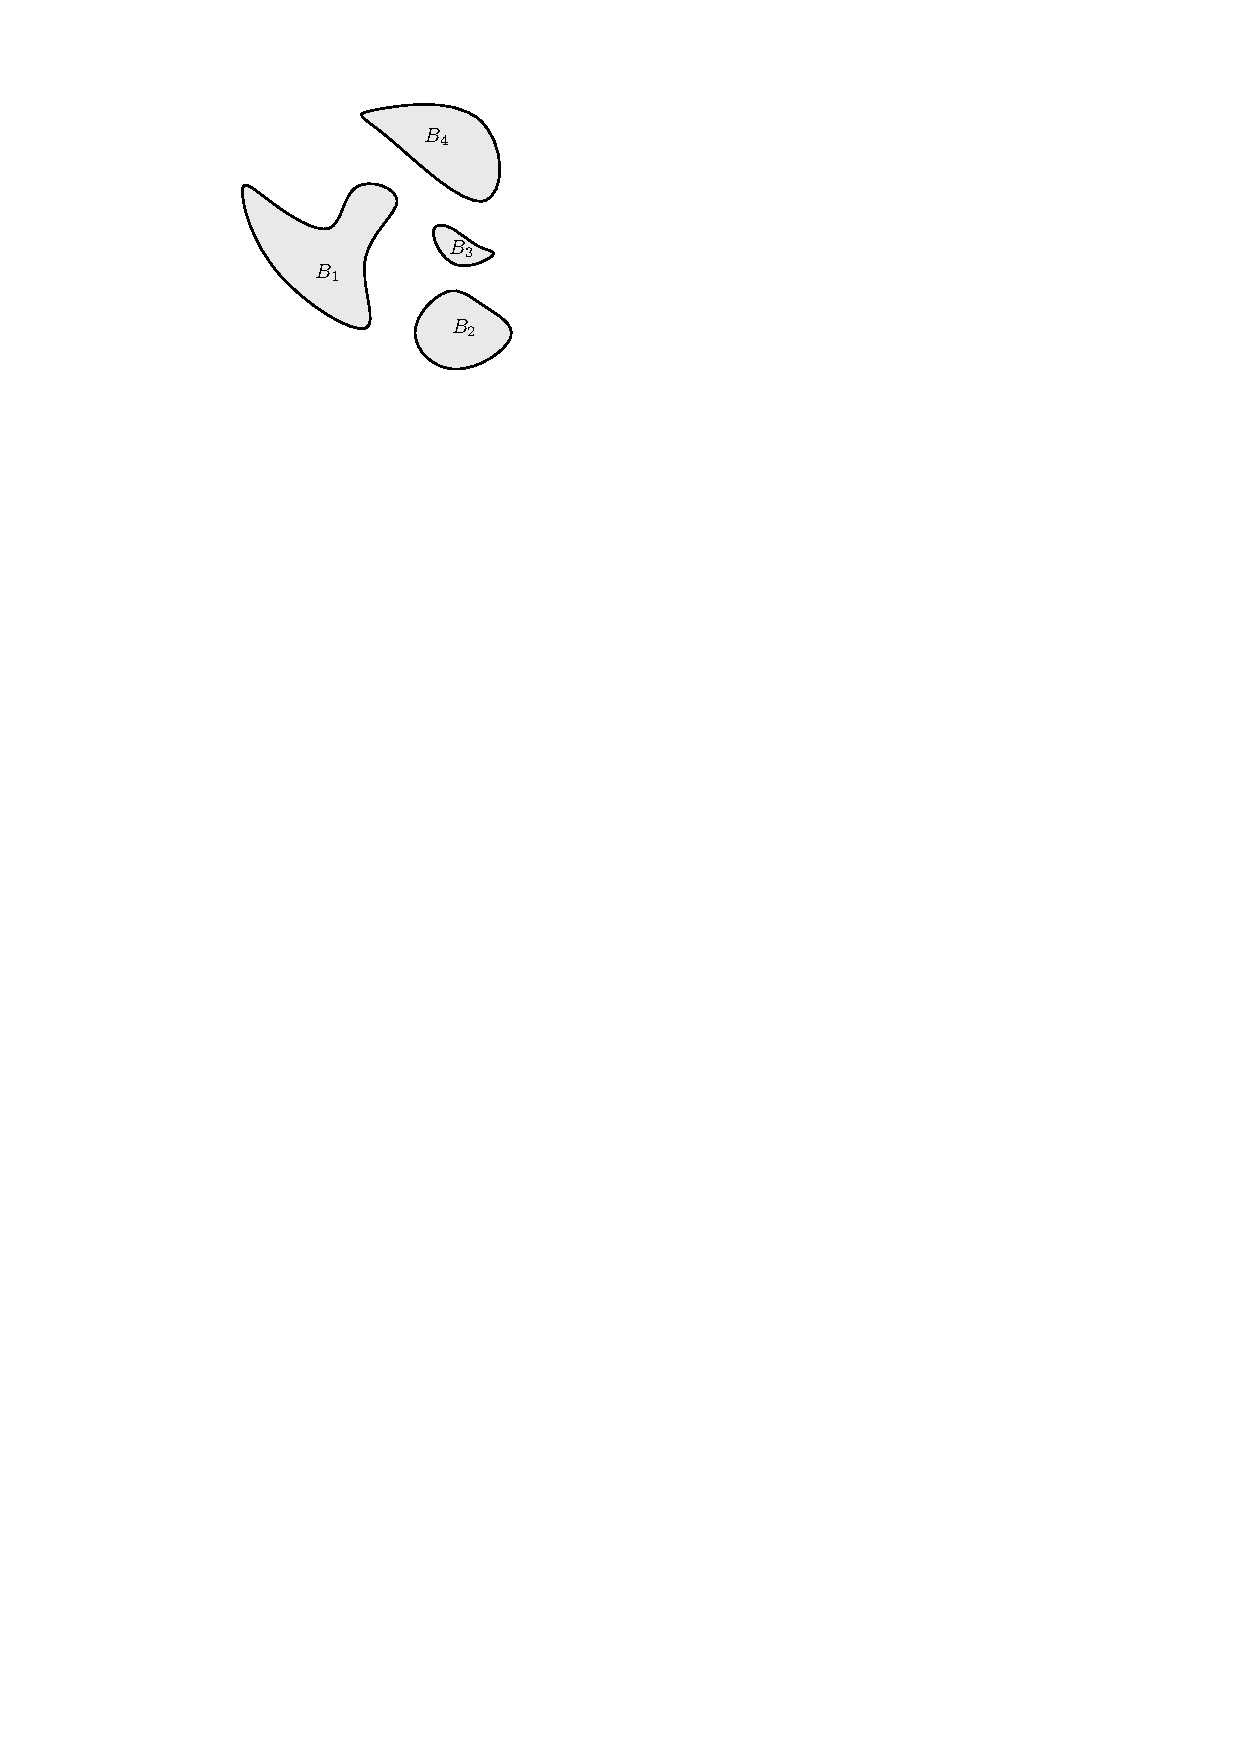
\includegraphics{ch02-bc-dimenze.pdf}
        \caption{Množina $B=\bigcup_{i=1}^4 B_i$}
        \label{subfig:bc-dimenze-pokryvana-mnozina}
    \end{subfigure}
    \qquad
    \begin{subfigure}{0.4\textwidth}
        \centering
        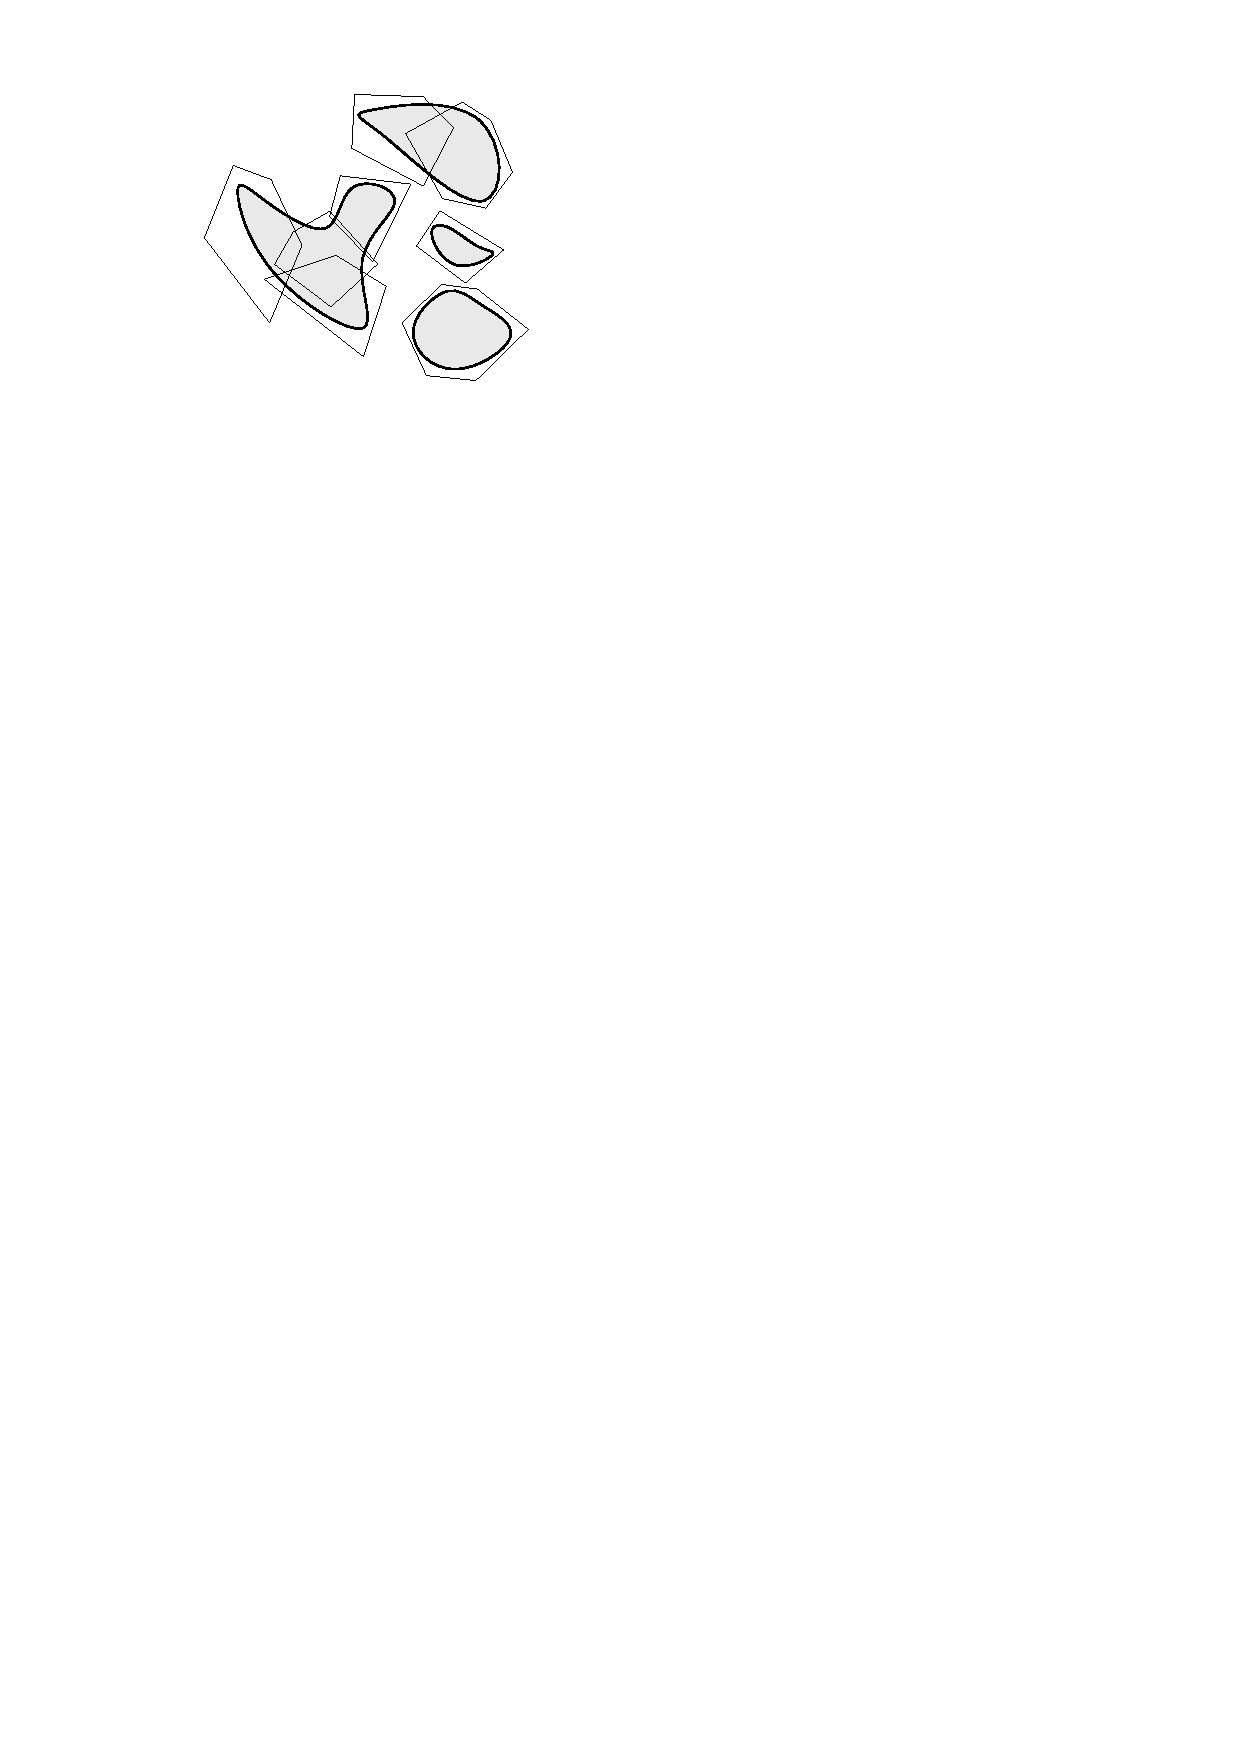
\includegraphics{ch02-bc-dimenze-delta-pokryti.pdf}
        \caption{$\delta$-pokrytí množiny $B$ (viz definice \ref{def:box-counting-dimenze})}
        \label{subfig:bc-dimenze-delta-pokryti}
    \end{subfigure}
    \qquad
    \begin{subfigure}{0.4\textwidth}
        \centering
        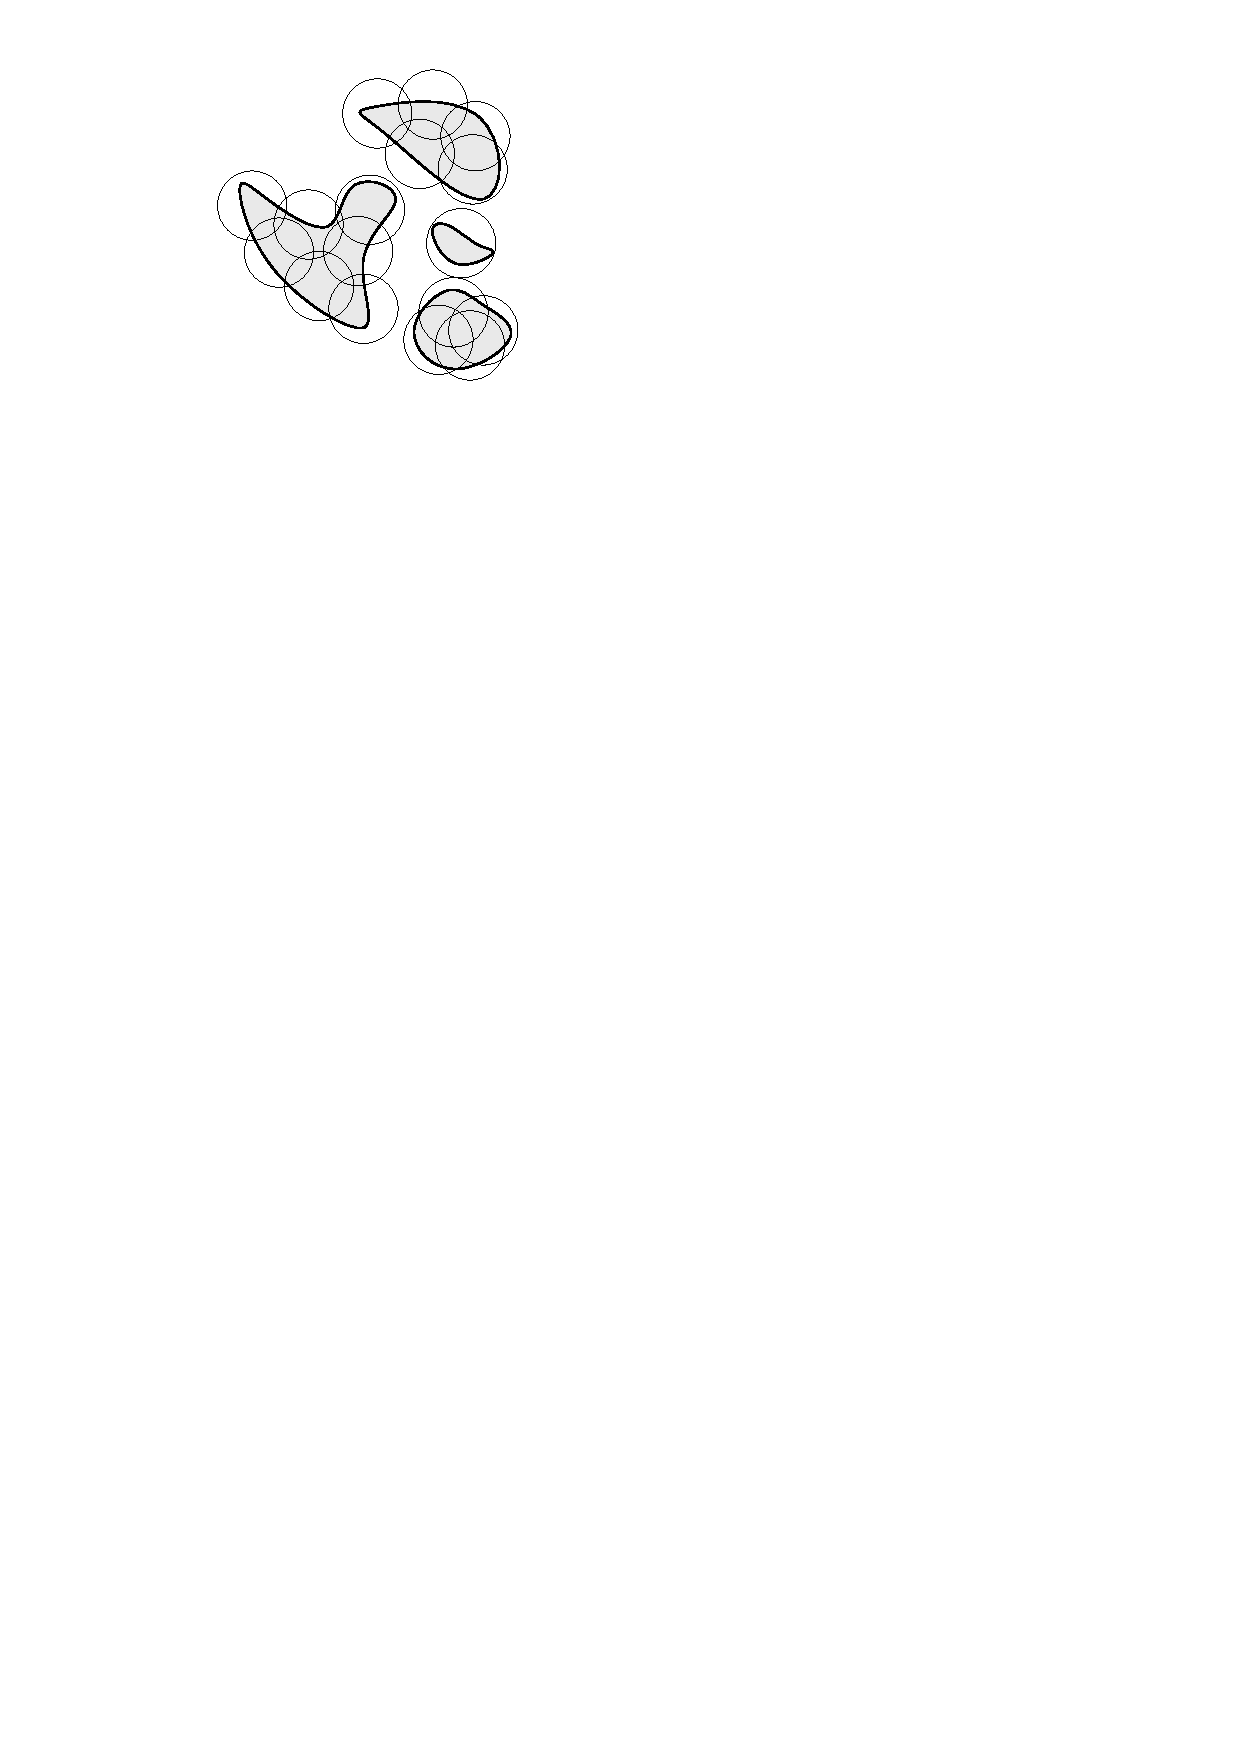
\includegraphics{ch02-bc-dimenze-pokryti-uz-koule.pdf}
        \caption{Pokrytí uzavřenými koulemi (viz bod \ref{thm:pokryti-delta-uz-koulemi})}
        \label{subfig:bc-dimenze-uz-koule}
    \end{subfigure}
    \qquad
    \begin{subfigure}{0.4\textwidth}
        \centering
        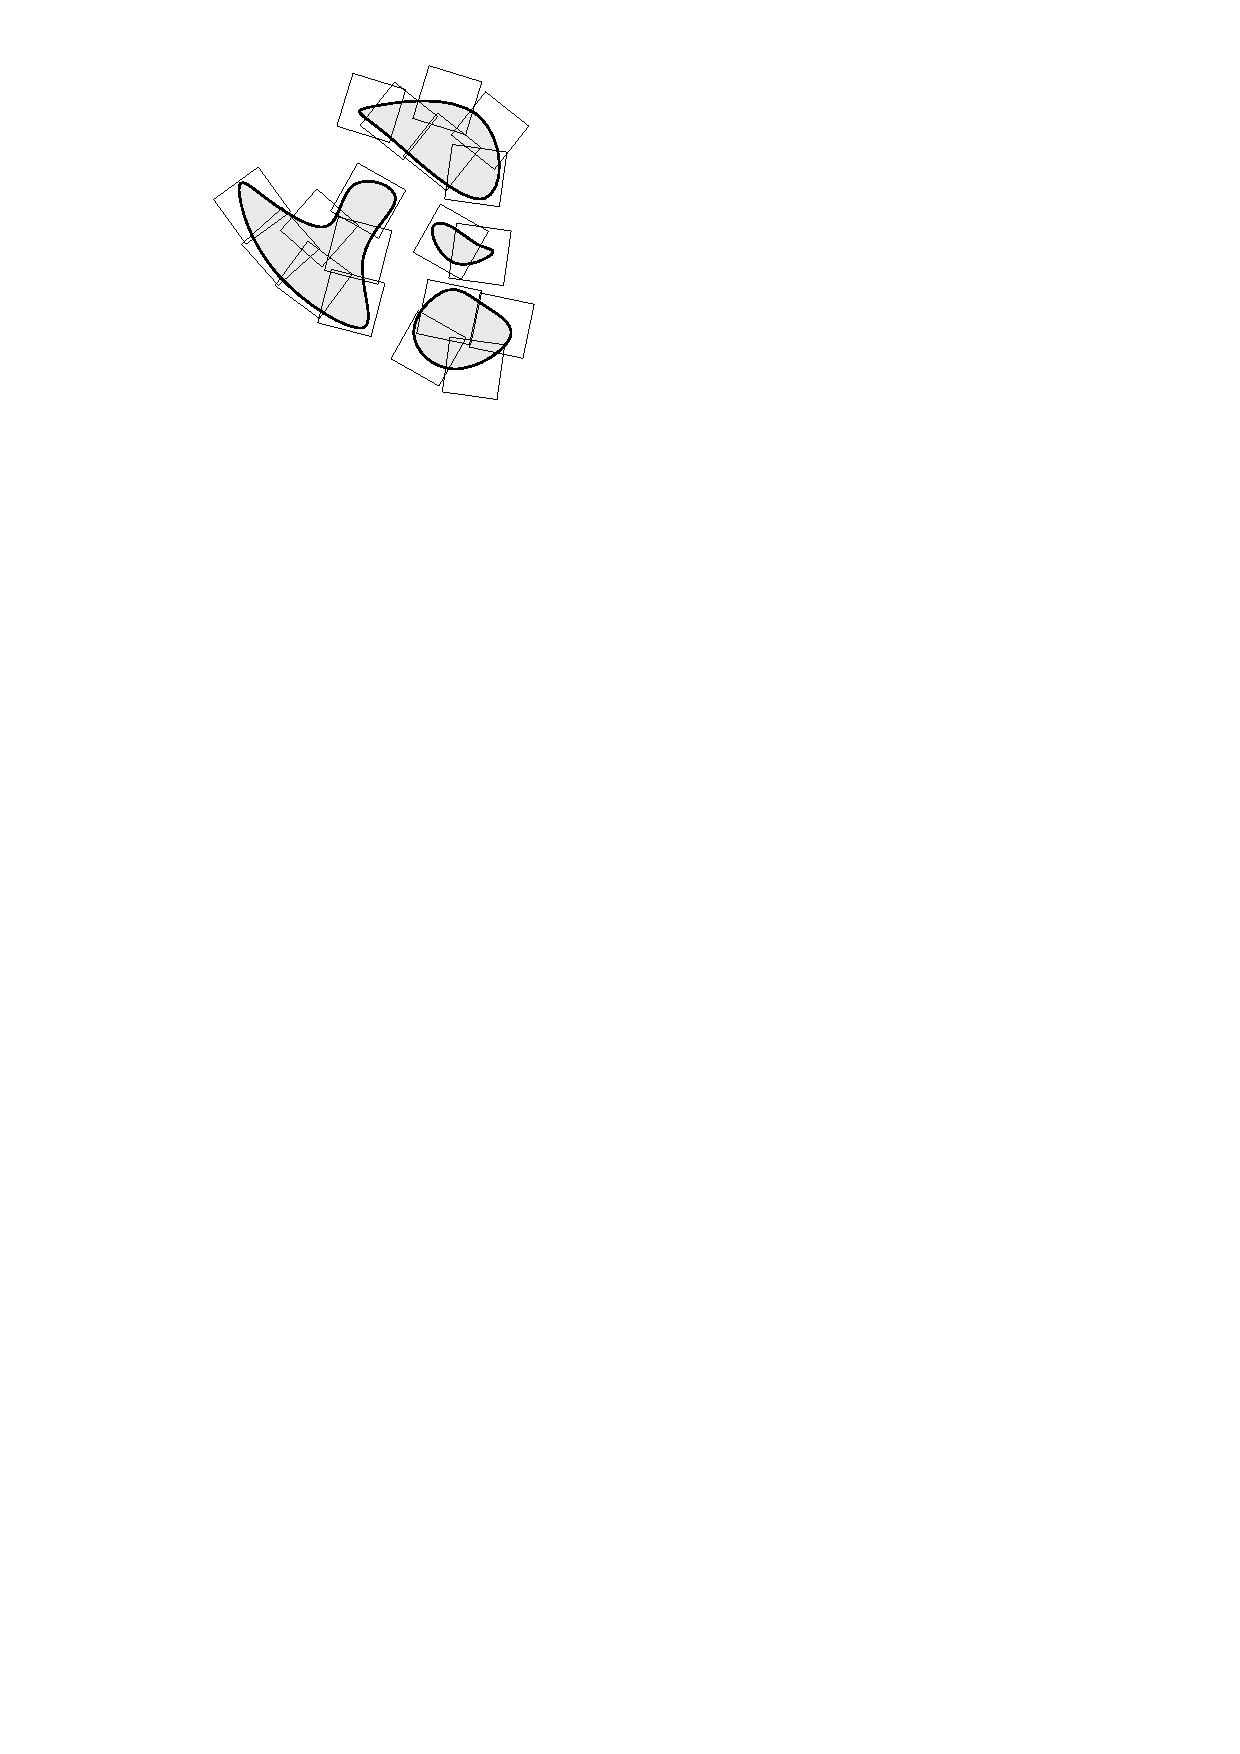
\includegraphics{ch02-bc-dimenze-pokryti-kvadry.pdf}
        \caption{Pokrytí pomocí kvádrů (viz bod \ref{thm:pokryti-delta-kvadry})}
        \label{subfig:bc-dimenze-kvadry}
    \end{subfigure}
    \qquad
    \begin{subfigure}{0.4\textwidth}
        \centering
        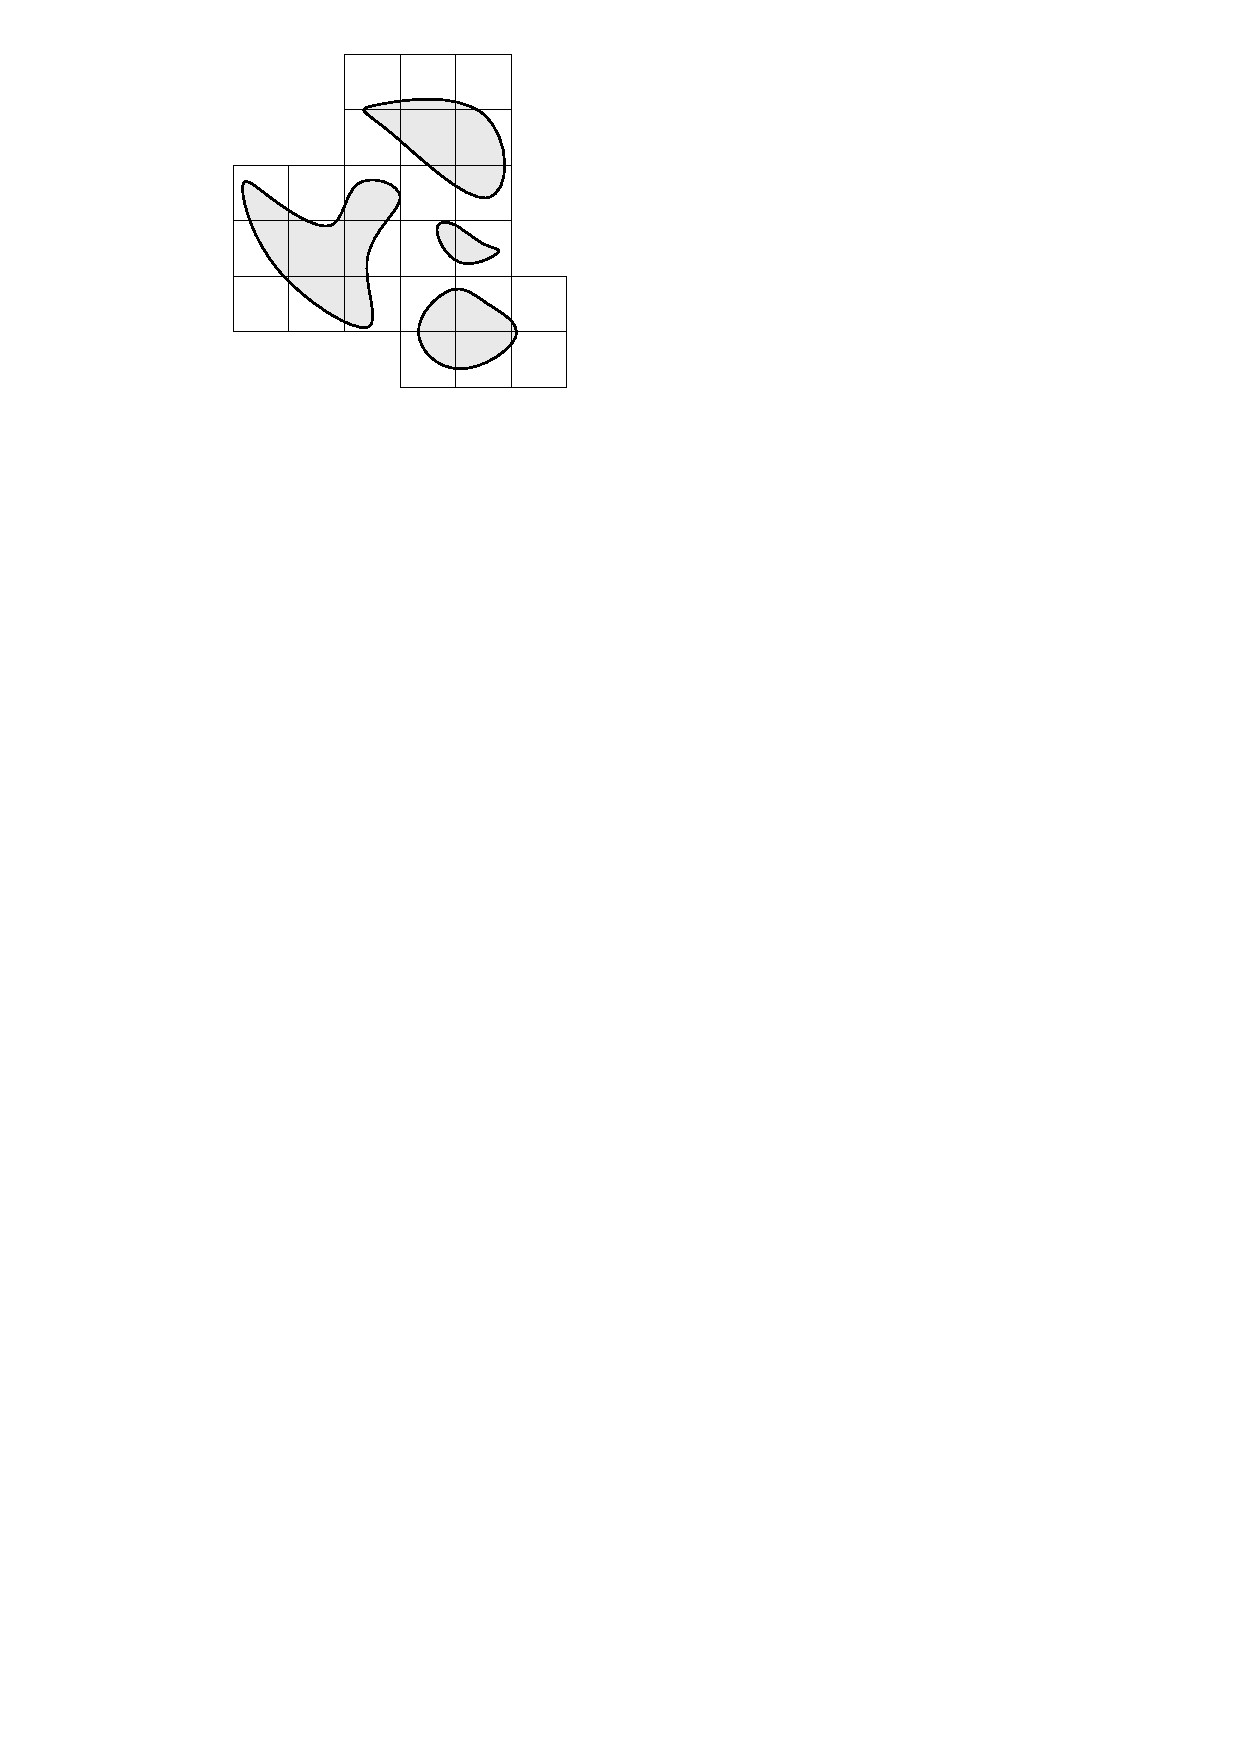
\includegraphics{ch02-bc-dimenze-pokryti-delta-sit.pdf}
        \caption{$\delta$-síť (viz bod \ref{thm:pokryti-delta-sit})}
        \label{subfig:bc-dimenze-delta-sit}
    \end{subfigure}
    \qquad
    \begin{subfigure}{0.4\textwidth}
        \centering
        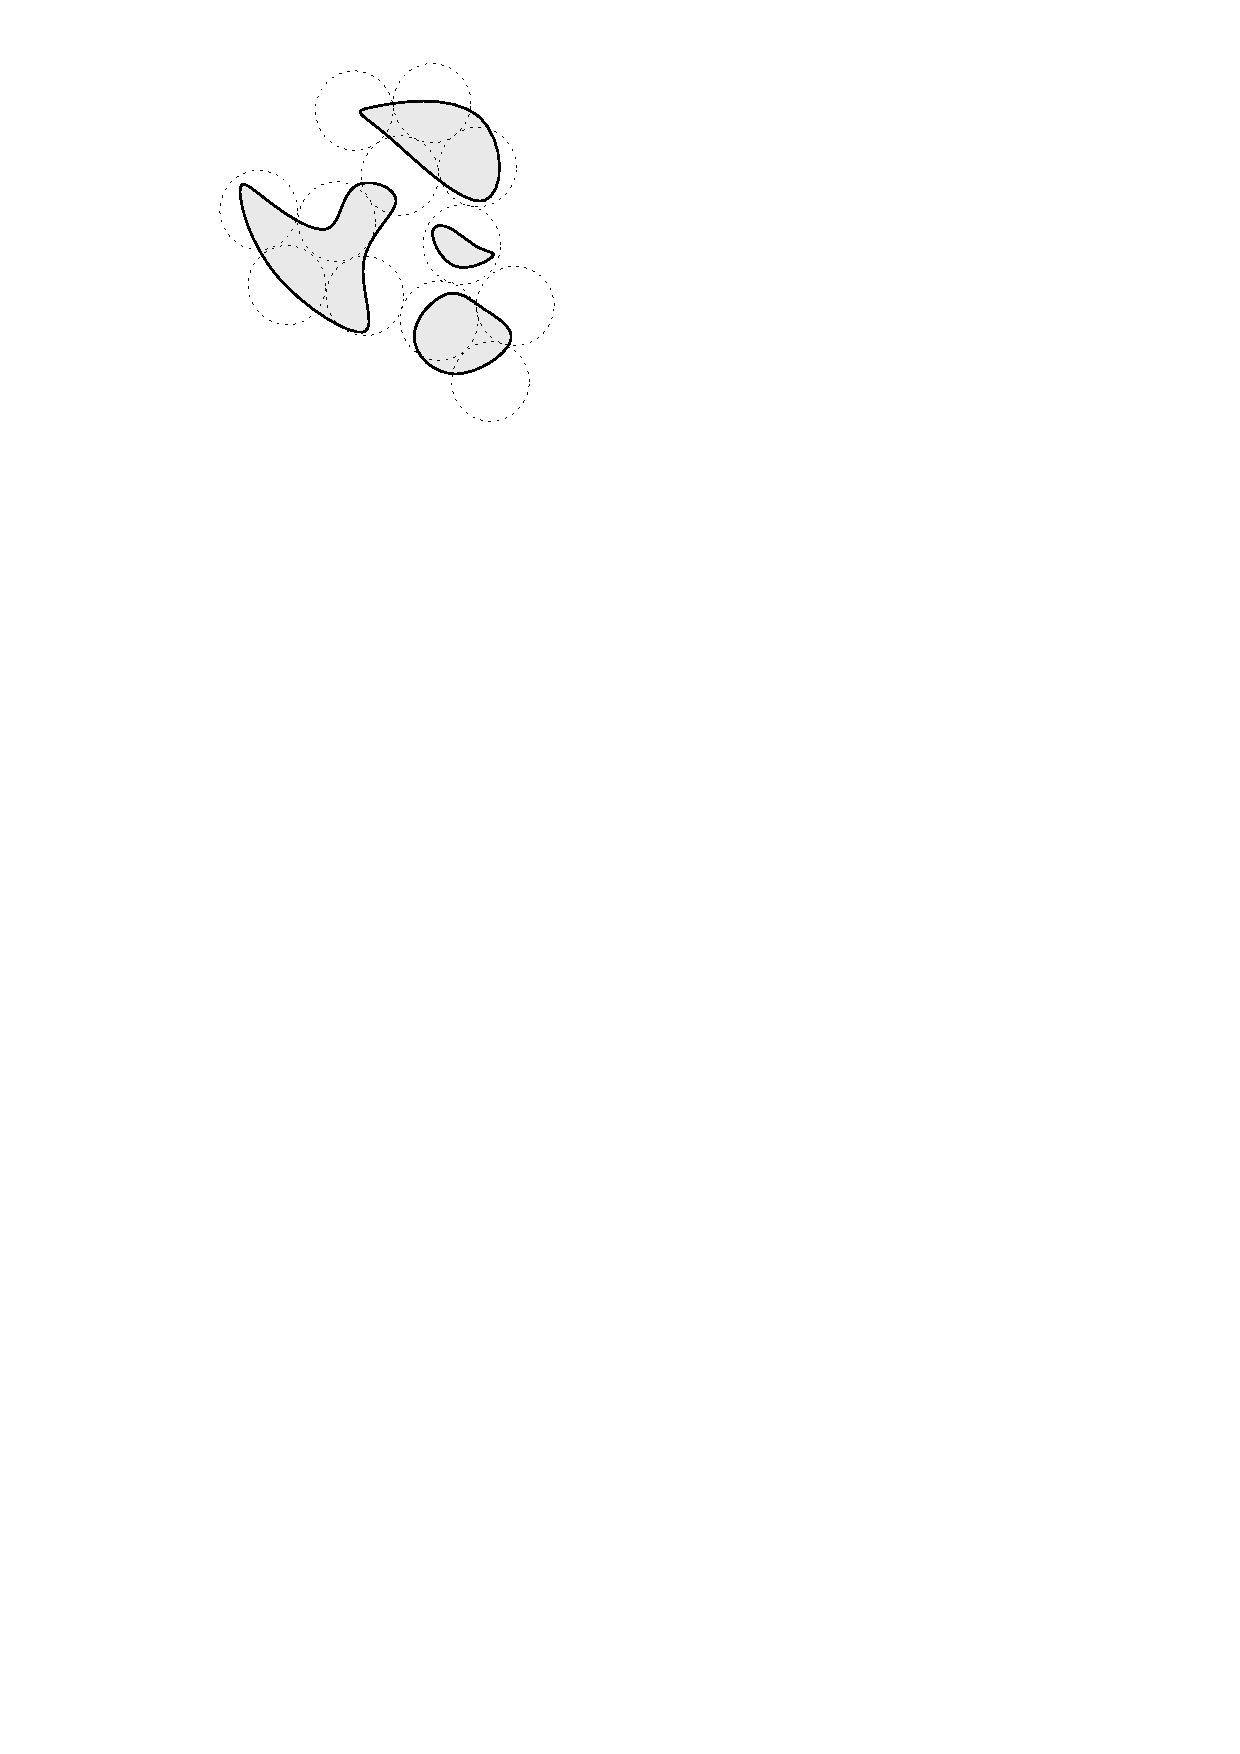
\includegraphics{ch02-bc-dimenze-pokryti-ot-koule.pdf}
        \caption{Pokrytí otevřenými po dvou disjunktními koulemi (viz bod \ref{thm:pokryti-delta-dis-ot-koulemi})}
        \label{subfig:bc-dimenze-ot-koule}
    \end{subfigure}
    \caption{Ilustrace věty \ref{thm:ekvivalentni-def-box-counting-dimenze} (Inspirováno \citep[str. 29]{Falconer2014})}
    \label{fig:ilustrace-definic-bc-dimenze}
\end{figure}

Zároveň body \ref{thm:pokryti-delta-kvadry} a \ref{thm:pokryti-delta-sit} nám dávají dobré opodstatnění názvu tohoto typu dimenze,~neboť v~podstatě zkoumáme pokrývání daného obrazce "kostkami". Při aproximacích box-counting dimenze obrazce $F\subset\R^2$ tak lze pracovat s~mřížkou čtverců o~libovolné straně $\delta>0$,~kdy $N_\delta(F)$ stanovíme jako počet čtverců,~které se překrývají se zkoumaným obrazcem $F$. Když se tedy zpět vrátíme k~otázce rozebírané v~úvodu tohoto textu týkající se délky pobřeží (viz kapitola \ref{chapter:uvod_do_fraktalu}),~lze jeho "fráktálnost" do jisté míry vyjádřit právě popsaným způsobem (viz obrázek \ref{fig:aproximace-delky-pobrezi-vb}).
\begin{figure}[h]
    \centering
    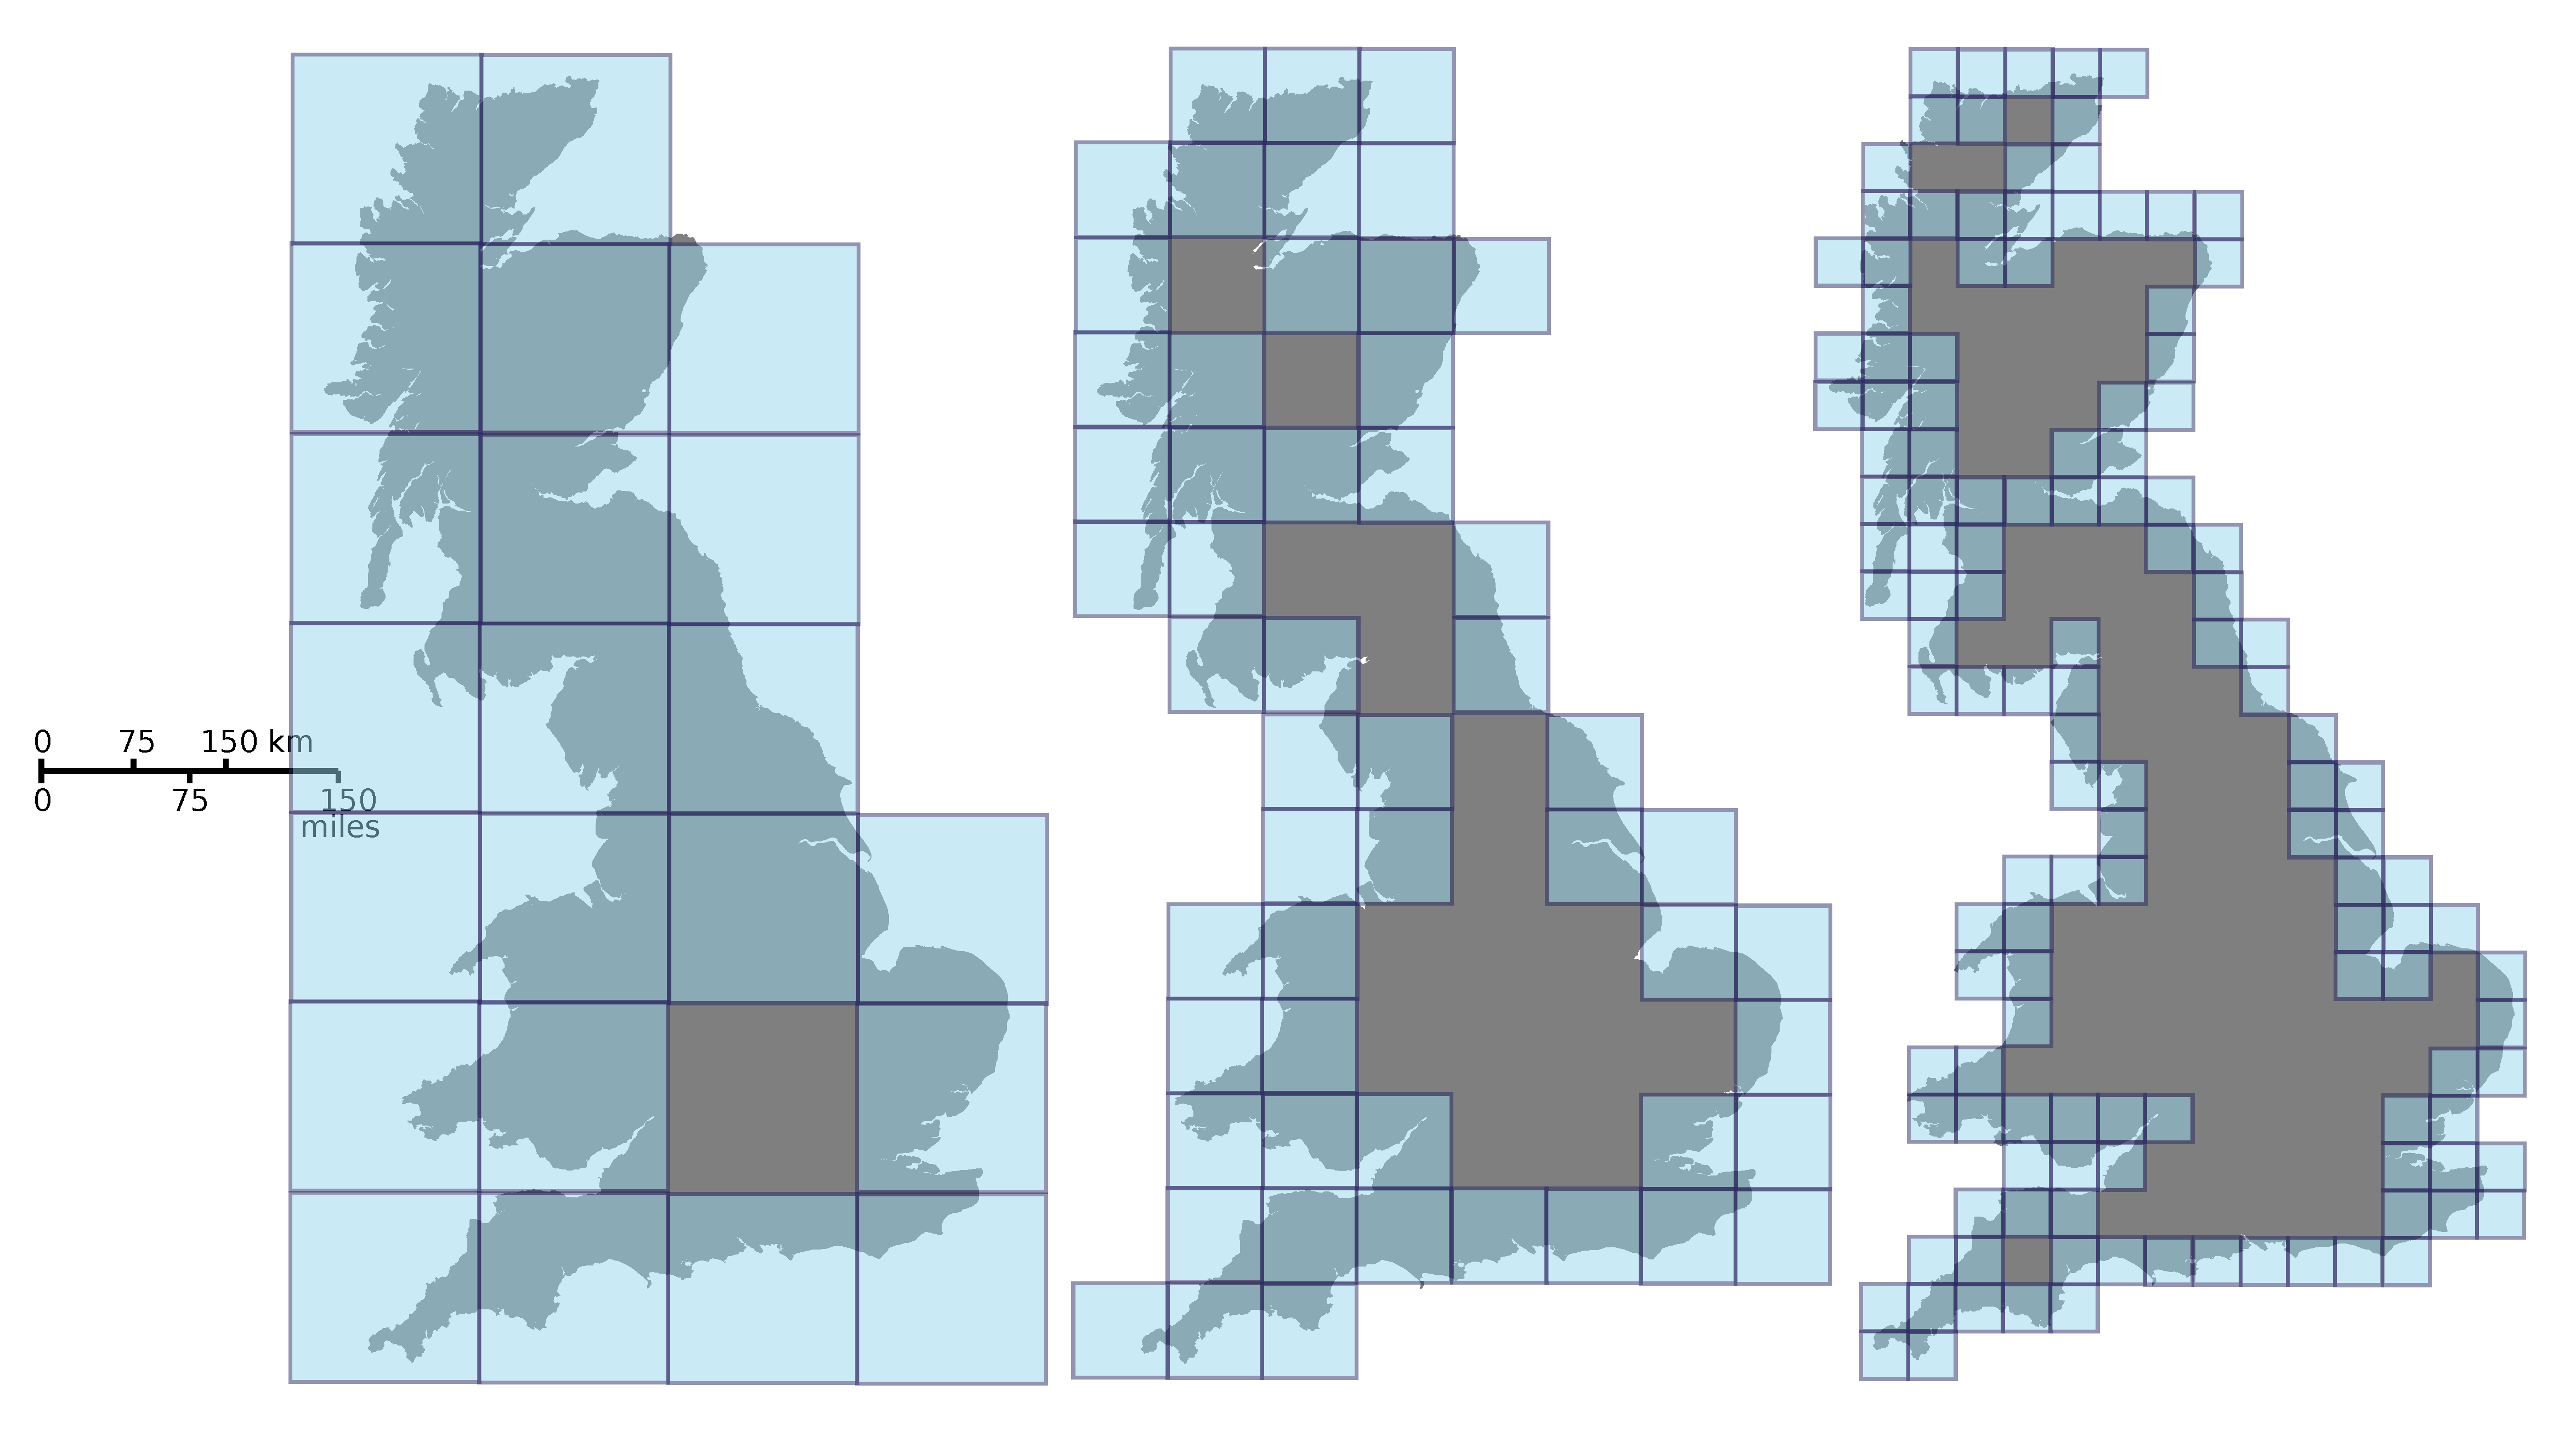
\includegraphics[width=\textwidth]{Great_Britain_Box.pdf}
    \caption[Aproximace box-counting dimenze pobřeží Velké Británie]{Aproximace box-counting dimenze pobřeží Velké Británie. Převzato z~Wikipedia Commons,~\url{https://en.wikipedia.org/wiki/Minkowski\%E2\%80\%93Bouligand\_dimension\#/media/File:Great\_Britain\_Box.svg}. Viz též \url{https://en.wikipedia.org/wiki/Minkowski\%E2\%80\%93Bouligand\_dimension}.}
    \label{fig:aproximace-delky-pobrezi-vb}
\end{figure}
Nyní se opět vrátíme k~fraktálům a výpočtům jejich dimenze,~čemuž jsme se věnovali již v~sekci \ref{sec:fraktalni_dimenze} kapitoly \ref{chapter:uvod_do_fraktalu},~konkrétně \ref{subsec:dimenze-fraktalu}. Tentokrát však budeme postupovat přímo podle definice box-counting dimenze \ref{def:box-counting-dimenze},~tedy budeme zvlášť zkoumat horní a dolní box-counting dimenzi.
\begin{example}[Cantorovo diskontinuum]\label{ex:cantorovo-diskontinuum}
    Formálně můžeme popsat Cantorovo diskontinuum $C$ jako průnik množin $C_k$ pro $k=0,1,2,\ldots$, přičemž
    \[C_k=\bigcup _{j=0}^{3^{k-1}-1}\left(\left\langle{\frac {3j+0}{3^{k}}},{\frac {3j+1}{3^{k}}}\right\rangle\cup \left\langle{\frac {3j+2}{3^{k}}},{\frac {3j+3}{3^{k}}}\right\rangle\right).\]
    $C_k$ tedy reprezentuje $k$-tou iteraci a~$C=\bigcap_{k=0}^\infty C_k$. Již jsme měli možnost se přesvědčit,~že tento fraktál má box-counting dimenzi $\ln{2}/\ln{3}$. Zkusme nyní výpočet zopakovat,~avšak vzlášť vypočítáme $\lowerdimB{C}$ a $\upperdimB{C}$ podíváme se,~zda se shodují.

    Jako první provedeme horní odhad. Je potřeba zvolit $\delta$ a na jeho základě dopočítat $N_\delta(C)$. V~$k$-té iteraci,~kde $k=0,1,2,\ldots$,~bude obecně $2^k$ intervalů,~každý o~délce $(1/3)^k$,~tedy pokud zvolíme $3^{-k}<\delta\leqslant 3^{-k+1}$,~pak intervaly o~délce nejvýše $\delta$ (viz věta \ref{thm:ekvivalentni-def-box-counting-dimenze},~bod \ref{thm:pokryti-delta-uz-koulemi}) tvoří $\delta$ pokrytí,~přičemž $N_\delta(C)\leqslant 2^k$. Tedy celkově pro $\delta$-pokrytí všech intervalů bude potřeba nejvýše $N_\delta(C)\leqslant 2^k$ intervalů $I_1,I_2,\ldots,I_{N_\delta(C)}$ o~průměru $3^{-k}<\diam{F_i}\leqslant 3^{-k+1}$ pro každé $i$. Z~toho dostáváme
    \[\upperdimB{C}=\limsup_{\delta\to 0}\dfrac{\ln{N_\delta(C)}}{-\ln{\delta}}\leqslant\limsup_{k\to\infty}\dfrac{\ln{2^k}}{-\ln{3^{-k+1}}}=\limsup_{k\to\infty}\dfrac{k\ln{2}}{(k-1)\ln{3}}=\dfrac{\ln{2}}{\ln{3}}.\]
    Naopak pokud uvážíme intervaly délky $3^{-k-1}\leqslant\delta<3^{-k}$,~pak každý z~nich má neprázdný průnik s~maximálně jedním intervalem $k$-té iterace $C$. Těch je,~jak již víme,~$2^k$,~tedy intervalů $I_1,I_2,\ldots,I_{N_\delta(C)}$ bude nejméně $2^k$ pro pokrytí $C$,~tzn. $N_\delta(C)\geqslant 2^k$. Tím dostáváme dolní odhad:
    \[\lowerdimB{C}=\liminf_{\delta\to 0}\dfrac{\ln{N_\delta(C)}}{-\ln{\delta}}\geqslant\liminf_{\delta\to 0}\dfrac{\ln{2^k}}{-\ln{3^{-k-1}}}=\liminf_{\delta\to 0}\dfrac{k\ln{2}}{(k+1)\ln{3}}=\dfrac{\ln{2}}{\ln{3}}.\]

    Protože $\lowerdimB{C}=\upperdimB{C}=\ln{2}/\ln{3}$,~tak box-counting dimenze Cantorova diskontinua je $\dimB{C}=\ln{2}/\ln{3}$. (Převzato z~\citep[str. 32]{Falconer2014})
\end{example}
Podobně bychom postupovali pro rovinné obrazce.
\begin{example}[Kochova křivka]\label{ex:kochova-krivka}
    Zde se zatím s~formální definicí nebudeme zatěžovat. Opět ukážene horní a~dolní odhad zvlášť. Kochovu křivku si označíme $K$.

    Obecně $k$-tá iterace Kochovy křivky bude obsahovat $4^n$ úseček,~každá o~délce $(1/3)^k$. Podobně jako v~předchozím příkladu \ref{ex:cantorovo-diskontinuum} zvolíme $3^{-k}<\delta\leqslant 3^{-k+1}$. Pokud si pro pokrytí zvolíme uzavřené koule
    \[K_\delta^1(x_1),K_\delta^2(x_2),\ldots,K_\delta^{N_\delta(K)}(x_{N_\delta(K)}),\;\text{kde}\;x_1,x_2,\ldots,x_{N_\delta(K)}\in\R^2\]
    pak $N_\delta(K)\leqslant 4^k$. Tedy
    \[\upperdimB{K}=\limsup_{\delta\to 0}\dfrac{\ln{N_\delta(K)}}{-\ln{K}}\leqslant\limsup_{k\to\infty}\dfrac{\ln{4^k}}{-\ln{3^{-k+1}}}=\limsup_{k\to\infty}\dfrac{k\ln{4}}{(k-1)\ln{3}}=\dfrac{\ln{4}}{\ln{3}}.\]

    Podobně pro dolní odhad uvážíme $3^{-k-1}\leqslant\delta<3^{-k}$. Vezmeme-li uzavřené koule $K_\delta^1(x_1),K_\delta^2(x_2),\ldots,K_\delta^{N_\delta(K)}(x_{N_\delta(K)})$,~pak žádný nemůže mít neprázdný průnik s~více než čtyřmi úsečkami,~tedy pro jejich pokrytí je zapotřebí alespoň $N_\delta(K)\geqslant 4^k/4=4^{k-1}$,~čímž dostáváme
    \[\lowerdimB{K}=\liminf_{\delta\to 0}\dfrac{\ln{N_\delta(K)}}{-\ln{K}}\geqslant\liminf_{k\to\infty}\dfrac{\ln{4^{k-1}}}{-\ln{3^{-k-1}}}=\liminf_{k\to\infty}\dfrac{(k-1)\ln{4}}{(k+1)\ln{3}}=\dfrac{\ln{4}}{\ln{3}}.\]
    Tzn.~$\dimB{K}=\ln{4}/\ln{3}$.
\end{example}
\begin{remark}
    Obecně množina $F$ skládající se z~$m$ disjunktních kopií sebe samotné v~měřítku $r$ má dimenzi $\dimB{F}=-\ln{m}/\ln{r}$.
\end{remark}
Nyní se podíváme ještě na jedno možné pojetí box-counting dimenze. Připomeňme,~že $\delta$-okolím množiny $F$ v~metrickém prostoru $(X,\rho)$ rozumíme
\[F_\delta=\set{x\in X\mid\exists y\in X: \rho(x,y)<\delta}.\]
Budeme nyní sledovat,~jak "rychle" se mění objem $F_\delta$ pro $\delta\to 0$. A~se zmínkou objemu nám zde do hry opět vstupuje Lebesgueova míra $\lambda_n$,~o níž jsme si povídali v~sekci \ref{sec:lebesgueova-mira}. Podívejme se nejdříve na několik příkladů.
\begin{itemize}
    \item Pro úsečku $u\subset\R^3$ o~délce $\ell$ lze objem jejího $\delta$-okolí stanovit jako
    \[\lambda_3(u)=\dfrac{4}{3}\pi \delta^3+\pi\delta^2\ell.\]
    Pokud však uvážíme $\delta$ dostatečně malé,~lze první člen zanedbat a psát
    \[\lambda_3(u)\approx\pi\ell\delta^2.\]
    \item V~případě uzavřené omezené množiny $F$ o~obsahu $A$ je objem $\lambda_3(F_\delta)\approx 2A\delta$.
    \item Pro kouli $B_r(x)\subset\R^3$,~kde $x\in\R^3$ a $r>0$ je objem
    \[\lambda_3((B_r(x))_\delta)=\dfrac{4}{3}\pi (r+\delta)^3=\dfrac{4}{3}\pi r^3+4\pi r^2\delta+4\pi r\delta^2+\dfrac{4}{3}\pi\delta^3\approx\dfrac{4}{3}\pi r^3.\]
    Změna objemu je v~tomto případě vzhledem k~$\delta$ zanedbatelná.
\end{itemize}
Můžeme si všimnout,~že v~každém případě odhad objemu vychází $\lambda_3(F)\approx c\delta^{3-s}$,~kde $c>0$ je závislé na původní míře $F$ a $s$ udává dimenzi. Obecněji pro množinu $F\subseteq\R^n$ bychom došli k~$\lambda_n(F)\approx c\delta^{n-s}$. Nyní,~podobně jako v~úvodu této sekce,~zkusme opět vyjádřit $s$:
\begin{align*}
    \ln{\lambda_n(F)}&\approx\ln{c}+(n-s)\ln{\delta}\\
    s\ln{\delta}&\approx n\ln{\delta}-\ln{\lambda_n(F)}+\ln{c}\\
    s&\approx n-\dfrac{\ln{\lambda_n(F)}}{\ln{\delta}}+\dfrac{\ln{c}}{\ln{\delta}}.
\end{align*}
Poslední člen bude v~limitě opět nulový.

Lze ukázat,~že $s$ není v~tomto případě nic jiného,~než již námi zkoumaná\linebreak{}box-counting dimenze. To si shrneme a dokážeme ve větě \ref{thm:bc-dimenze-lebesgueova-mira}.
\begin{theorem}\label{thm:bc-dimenze-lebesgueova-mira}
    Nechť $F\in\mathcal{L}^n$ je uzavřená a omezená. Pak platí: 
    \begin{enumerate}[label=(\roman*)]
        \item $\lowerdimB{F}=n-\liminf\limits_{\delta\to 0}\dfrac{\ln{\lambda_n(F_\delta)}}{\ln{\delta}}$,
        \item $\upperdimB{F}=n-\limsup\limits_{\delta\to 0}\dfrac{\ln{\lambda_n(F_\delta)}}{\ln{\delta}}$.
    \end{enumerate}
\end{theorem}
\begin{proof}
    V~rámci důkazu využijeme větu \ref{thm:ekvivalentni-def-box-counting-dimenze}.

    Mějme $F\in\mathcal{L}^n$ omezenou a uzavřenou. Označme $v_n$ objem jednotkové koule $K_1(x)$\footnote{Objem koule v~$\R^n$ lze vyjádřit vztahem
    \[V_n(r)=\dfrac{\pi^{n/2}}{\Gamma\left(\frac{n}{2}+1\right)}r^n,\]
    kde $\Gamma$ je tzv. \emph{gamma funkce}. Se vzorcem však dále v~textu pracovat nebudeme.
    } v~$\R^n$ pro $x\in\R^n$ libovolné. Dále mějmě pokrytí
    \[\mathcal{K}=\set{K_\delta^1(x_1),K_\delta^2(x_2),\ldots,K_\delta^{N_\delta(F)}(x_{N_\delta(F)})}\]
    množiny $F$,~kde $0<\delta<1$ a $x_j\in F$ pro každé $1\leqslant j\leqslant N_\delta(F)$. Pak lze zvolit pokrytí
    \[\mathcal{K}^\prime=\set{K_{2\delta}^1(x_1),K_{2\delta}^2(x_2),\ldots,K_{2\delta}^{N_\delta(F)}(x_{N_\delta(F)})},\]
    tzn.~$\mathcal{K}$ je zjemnění pokrytí $\mathcal{K}^\prime$. Zároveň však platí,~že $\mathcal{K}$ je i~pokrytím $F_\delta$. Pro libovolné $x\in F_\delta$ existuje totiž $y\in F$,~takové,~$\rho(x,y)<\delta$. Tedy pro dané $y$ existuje nějaká koule $K_\ell(x_\ell)\in\mathcal{K}$,~taková,~že $y\in K_\ell(x_\ell)$,~což znamená,~že
    \[\rho(x_\ell,y)\leqslant\rho(x_\ell,x)+\rho(x,y)\leqslant\delta+\delta=2\delta.\]
    Tzn.~míru $F$ lze zhora odhadnout jako
    \[\lambda_n(F_\delta)\leqslant N_\delta(F)v_n(2\delta)^n.\]
    Úpravou získáme:
    \begin{align*}
        \ln{\lambda_n(F_\delta)}&\leqslant n\ln{\delta}+\ln{N_\delta(F)}+\ln{2^nv_n}\\
        \dfrac{\ln{\lambda_n(F_\delta)}}{-\ln\delta}&\leqslant -n+\dfrac{\ln{N_\delta(F)}}{-\ln\delta}+\dfrac{\ln{2^nv_n}}{-\ln\delta},
    \end{align*}
    tedy v~limitě
    \[\liminf_{\delta\to 0}\dfrac{\ln\lambda_n(F_\delta)}{-\ln\delta}\leqslant -n+\lowerdimB{F}.\]
    K~odhadu $\upperdimB{F}$ lze dospět analogicky.

    Nyní uvažujme po dvou disjunktní otevřené koule $B_\delta^j(x_j)$,~kde $x_j\in F$ pro $1\leqslant j\leqslant N_\delta(F)$. Pak součtem jejich objemů získáme
    \[N_\delta(F)v_n\delta^n\leqslant\lambda_n(F_\delta).\]
    Obdobnou úpravou této nerovnosti získáme požadovanou nerovnost.
\end{proof}
Zkusme si aplikaci věty ilustrovat opět na příkladu fraktálu.
\begin{example}[Cantorovo diskontinuum potřetí]
    Pro Cantorovo diskontinuum $C$ v~$k$-té iteraci lze odhadnout délku $C_\delta$ pro $3^{-k}\leqslant\delta\leqslant 3^{-k+1}$ jako
    \[\lambda_1(C_\delta)\leqslant2^k\cdot 2\delta=2^{k+1}3^{-k+1}.\]
    Tedy podle věty \ref{thm:bc-dimenze-lebesgueova-mira}
    \begin{align*}
        \upperdimB{C}&=n-\limsup_{\delta\to 0}\dfrac{\ln{\lambda_1(C_\delta)}}{\ln{\delta}}\leqslant1-\limsup_{k\to\infty}\dfrac{\ln{2^{k+1}3^{-k+1}}}{\ln{3^{-k+1}}}\\
        &=\limsup_{k\to\infty}\dfrac{(k+1)\ln{2}}{(k-1)\ln{3}}=\dfrac{\ln{2}}{\ln{3}}.
    \end{align*}

    Podobně zvolíme-li $3^{-k-1}\leqslant\delta\leqslant 3^{-k}$,~pak
    \[\lambda_1(C_\delta)\geqslant 2^{k+1}3^{-k-1}\]
    a tedy
    \begin{align*}
        \lowerdimB{C}&=n-\liminf_{\delta\to 0}\dfrac{\ln{\lambda_1(C_\delta)}}{\ln{\delta}}\geqslant 1-\liminf_{k\to\infty}\dfrac{\ln{2^{k+1}3^{-k-1}}}{\ln{3^{-k-1}}}\\
        &=\liminf_{k\to\infty}\dfrac{(k+1)\ln{2}}{(k+1)\ln{3}}=\dfrac{\ln{2}}{\ln{3}}.
    \end{align*}
\end{example}

\subsection{Vlastnosti}\label{subsec:vlastnosti-bc-dimenze}

V minulé podsekci \ref{subsec:definice-a-vypocet-bc-dimenze} jsme se bavili o~možnostech pojetí box-counting dimenze. S~tím souvisely zejména pak věty \ref{thm:ekvivalentni-def-box-counting-dimenze} a \ref{thm:bc-dimenze-lebesgueova-mira}. Nyní trochu blíže ještě prozkoumáme některé její vlastnosti,~na něž se podíváme ve větě \ref{thm:vlastnosti-bc-dimenze}.
\begin{theorem}[Vlastnosti box-counting dimenze]\label{thm:vlastnosti-bc-dimenze}
    Nechť jsou dány $F,G\subseteq\R^n$.
    \begin{enumerate}[label=(\roman*)]
        \item\label{thm:monotonie-bc-dimenze} Pokud $G\subseteq F$,~pak $\lowerdimB{G}\leqslant\lowerdimB{F}$ a $\upperdimB{G}\leqslant\upperdimB{F}$.\rightnote{monotonie}
        \item\label{thm:rozsah-hodnot-bc-dimenze} Je-li $F\neq\emptyset$ omezená,~pak $0\leqslant\lowerdimB{F}\leqslant\upperdimB{F}\leqslant n$. \rightnote{rozsah hodnot}
        \item\label{thm:stabilita-bc-dimenze} $\upperdimB(F\cup G)=\max\set{\upperdimB{F},\upperdimB{G}}$.\rightnote{stabilita}
    \end{enumerate}
\end{theorem}
\begin{proof}
    \begin{enumerate}[label=\textit{(\roman*)}]
        \item Plyne triviálně z~faktu,~že pro libovolné $\delta>0$ je $N_\delta(G)\leqslant N_\delta(F)$,~neboť každé $\delta$-pokrytí $\mathcal{F}\supset F$ je zároveň $\delta$-pokrytím $G$.
        \item První dvojice nerovností je zjevná z~definice (viz \ref{def:box-counting-dimenze}). Pro třetí nerovnost zvolme kvádr $I$,~takový,~že $F\subset I$. Zvolíme-li $\delta>0$ a $\delta$-síť $\mathcal{D}$,~pak podle věty \ref{thm:ekvivalentni-def-box-counting-dimenze} je
        \[N_\delta(F)\leqslant N_\delta(I)=\left|\set{J\;\middle|\;J\cap I\neq\emptyset\;,\;J\in\mathcal{D}}\right|\leqslant c\delta^{-n},\]
        kde $c>0$. Tedy
        \[\upperdimB{F}\leqslant\upperdimB{I}=\limsup_{\delta\to 0}\dfrac{\ln{N_\delta(I)}}{-\ln{\delta}}\leqslant\limsup_{\delta\to 0}\dfrac{\ln{c\delta^{-n}}}{-\ln{\delta}}=n.\]
        \item Pro $\delta>0$ volme $\delta$-pokrytí $\mathcal{F}\supset F$ a $\mathcal{G}\supset G$. Je celkem zjevné,~že $N_\delta(F\cup G)\leqslant N_\delta(F)+N_\delta(G)$,~neboli
        \begin{align*}
            \ln(N_\delta(F)+N_\delta(G))&\leqslant \ln\left(2\max\set{N_\delta(F),N_\delta(G)}\right)\\
            &=\ln{2}+\ln\left(\max\set{N_\delta(F),N_\delta(G)}\right).
        \end{align*}
        Tedy
        \begin{align*}
            \upperdimB(F\cup G)&\leqslant\limsup_{\delta\to 0}\left(\dfrac{\ln{2}}{-\ln{\delta}}+\dfrac{\ln\left(\max\set{N_\delta(F),N_\delta(G)}\right)}{-\ln{\delta}}\right)\\
            &\leqslant\limsup_{\delta\to 0}\dfrac{\ln\left(\max\set{N_\delta(F),N_\delta(G)}\right)}{-\ln{\delta}}\\
            &=\limsup_{\delta\to 0}\left(\max\set{\dfrac{\ln{N_\delta(F)}}{-\ln{\delta}},\dfrac{\ln{N_\delta(G)}}{-\ln{\delta}}}\right)\\
            &\leqslant\max\set{\limsup_{\delta\to 0}\dfrac{\ln{N_\delta(F)}}{-\ln{\delta}},\limsup_{\delta\to 0}\dfrac{\ln{N_\delta(G)}}{-\ln{\delta}}}\\
            &=\max\set{\upperdimB{F},\upperdimB{G}}.
        \end{align*}
        Opačná nerovnost plyne z~faktu,~že $F\subset F\cup G$ a $G\subset F\cup G$,~tedy
        \[\upperdimB(F\cup G)\geqslant\upperdimB{F}\;\text{a}\;\upperdimB(F\cup G)\geqslant\upperdimB{G}\]
        podle bodu \ref{thm:monotonie-bc-dimenze},~neboli
        \[\upperdimB(F\cup G)=\max\set{\upperdimB{F},\upperdimB{G}}.\]
    \end{enumerate}
\end{proof}
(Převzato a upraveno z~\citep[str. 35]{Falconer2014}.)

Poslední bod \ref{thm:stabilita-bc-dimenze} tvrzení \ref{thm:vlastnosti-bc-dimenze} lze pochopitelně rozšířit indukcí. Čtenář se sám může přesvědčit,~že se jedná o~relativně jednoduché cvičení.
\begin{corollary}\label{cor:stabilita-bc-dimenze-obecne}
    Pro $F_1,F_2,\ldots,F_m\subseteq\R^n$ platí:
    \[\upperdimB\left(\bigcup_{i=1}^m F_i\right)=\max\set{\upperdimB{F_j}\mid 1\leqslant j\leqslant m}.\]
\end{corollary}
\begin{proof}
    Pro $m=1$ a $m=2$ víme,~že tvrzení platí. Pro $m+1$ lze psát:
    \begin{align*}
        \upperdimB\left(\bigcup_{i=1}^{m+1}F_i\right)&=\upperdimB\left(\left(\bigcup_{i=1}^{m}F_i\right)\cup F_{m+1}\right)\\
        &=\max\set{\upperdimB\left(\bigcup_{i=1}^{m+1}F_i\right),\upperdimB{F_{m+1}}}\\
        &\stackrel{\text{I.P.}}{=}\max\set{\max\set{\upperdimB{F_i}\mid 1\leqslant i\leqslant m},\upperdimB{F_{m+1}}}\\
        &=\max\set{\upperdimB{F_j}\mid 1\leqslant j\leqslant m+1}.
    \end{align*}
\end{proof}

Jako poslední se ještě nabízí otázka,~jak se bude dimenze $\dimB$ chovat vůči zobrazením. V~tomto kontextu pro nás budou relevantní především \emph{lipschitzovská}\index{lipschitzovské zobrazení} a \emph{bilipschitzovská zobrazení}\index{bilipschitzovské zobrazení}. Připomeňme,~že lipschitzovské zobrazení je takové zobrazení $\mapping{f}{X}{Y}$ mezi metrickými prostory $(X,\rho_1)$ a $(Y,\rho_2)$,~že existuje konstanta $K>0$, taková, že pro každé $x,y\in X$ platí
\[\rho_2(f(x),f(y))\leqslant K\rho_1(x,y).\]
Pokud navíc platí,~že existují konstanty $K_1,K_2>0$,~takové,~že platí
\[K_1\rho_1(x,y)\leqslant\rho_2(f(x),f(y))\leqslant K_2\rho_1(x,y),\]
pak $f$ nazýváme bilipschitzovské.

Než se však podíváme na samotný vztah box-counting dimenze a lipschitzovských,~resp. bilipschitzovských zobrazení,~dokážeme si jedno jednoduché\linebreak{}lemma,~které později využijeme.
\begin{lemma}\label{lem:lipschitzovska-zobrazeni-a-bijekce}
    Nechť $(X,\rho_1),(Y,\rho_2)$ jsou metrické prostory a zobrazení $\mapping{f}{X}{Y}$ je bilipschitzovské. Pak $\mapping{f^\prime}{X}{f(X)}$ je bijekce.
\end{lemma}
\begin{proof}
    Podle předpokladu je $f$ bilipschitzovské zobrazení,~tedy i~$f^\prime$ je bilipschitzovské,~tedy existují pro konstanty $K_1,K_2>0$,~takové,~že
    \[K_1\rho_1(x,y)\leqslant\rho_2(f^\prime(x),f^\prime(y))\leqslant K_2\rho_1(x,y),\;x,y\in X.\]
    Surjektivita zobrazení $f^\prime$ je zřejmá z~její definice. Pro spor předpokládejme,~že $f^\prime$ není injektivní,~tedy existují $x,y\in X$,~taková,~že $x\neq y$ a $f^\prime(x)=f^\prime(y)$. Pak
    \[0<K_1\rho_1(x,y)\leqslant\rho_2(f^\prime(x),f^\prime(y))=0,\]
    což je spor.
\end{proof}

V našem případě se nyní dále omezíme,~stejně jako předtím,~pouze na prostor $\R^n$.

\begin{theorem}\label{thm:bc-dimenze-bi-lipschitzovska-zobrazeni}
    Nechť jsou dány metrické prostory $(\R^n,\rho_n)$ a $(\R^m,\rho_m)$,~zobrazení $\mapping{f}{\R^n}{\R^m}$ a $F\subseteq\R^n$. Platí:
    \begin{enumerate}[label=(\roman*)]
        \item\label{thm:bc-dimenze-lipschitz} Je-li $f$ lipschitzovské,~pak
        \[\lowerdimB{f(F)}\leqslant\lowerdimB{F}\;\text{a}\;\upperdimB{f(F)}\leqslant\upperdimB{F}.\]
        \item\label{thm:bc-dimenze-bilipschitz} Je-li $f$ bilipschitzovské,~pak
        \[\lowerdimB{f(F)}=\lowerdimB{F}\;\text{a}\;\upperdimB{f(F)}=\upperdimB{F}.\]
    \end{enumerate}
\end{theorem}
\begin{proof}
    Máme tedy metrické prostory $(\R^n,\rho_n)$,~$(\R^m,\rho_m)$,~zobrazení $\mapping{f}{\R^n}{\R^m}$ a $F\subseteq\R^n$.
    \begin{enumerate}[label=\textit{(\roman*)}]
        \item Jako první si všimneme,~že je-li $\mathcal{F}=\set{F_1,F_2,\ldots}$ $\delta$-pokrytí,~množiny $F$,~kde $\delta>0$,~pak je jím i~systém
        \[\mathcal{F}^\prime=\set{F\cap F_1,F\cap F_2,\ldots}.\]
        Podle předpokladu je $f$ lipschitzovské,~tzn. pro každé $x,y\in\R^n$ je
        \[\rho_m(f(x),f(y))\leqslant K\rho_n(x,y),\;K>0.\]
        Speciálně tak platí i~$\diam(f(F\cap F_i))\leqslant K\diam(F\cap F_i)$ pro každé $i$,~a tedy
        \[\diam(f(F\cap F_i))\leqslant K\diam(F\cap F_i)\leqslant K\diam{F_i}\leqslant K\delta.\]
        Z~toho plyne,~že $\mathcal{G}=\set{f(F\cap F_1),f(F\cap F_2),\ldots}$ tvoří $K\delta$-pokrytí množiny $f(F)$. Tedy máme,~že $N_{K\delta}(f(F))\leqslant N_\delta(F)$. Po úpravě
        \[\dfrac{\ln{N_{K\delta}(f(F))}}{-\ln{\delta}}\leqslant\dfrac{\ln{N_\delta(F)}}{-\ln{\delta}}.\]
        Tedy celkově
        \begin{align*}
            \upperdimB{f(F)}&=\limsup_{\delta\to 0}\dfrac{\ln{N_{K\delta}(f(F))}}{-\ln{K\delta}}=\limsup_{\delta\to 0}\dfrac{\ln{N_{K\delta}(f(F))}}{-\ln{\delta}}\cdot\dfrac{\ln{\delta}}{\ln{K\delta}}\\
            &\leqslant\limsup_{\delta\to 0}\dfrac{\ln{N_{\delta}(f(F))}}{-\ln{\delta}}\cdot\dfrac{\ln{\delta}}{\ln{K\delta}}=\limsup_{\delta\to 0}\dfrac{\ln{N_{\delta}(f(F))}}{-\ln{\delta}}\\
            &=\upperdimB{F}.
        \end{align*}
        Nerovnost pro $\lowerdimB{f(F)}$ obdržíme analogicky.
        \item Je-li $f$ bilipschitzovské,~pak podle lemmatu \ref{lem:lipschitzovska-zobrazeni-a-bijekce} je $\mapping{g}{\R^n}{f(\R^n)}$ bijekce a existuje inverzní zobrazení $\mapping{g^{-1}}{f(\R^n)}{\R^n}$. Volme $u,v\in f(\R^n)$ libovolně a položme $x=g^{-1}(u),y=g^{-1}(v)$. Pak
        \[K_1\rho_n(x,y)=K_1\rho_n(g^{-1}(u),g^{-1}(v))\leqslant\rho_m(g(g^{-1}(u)),g(g^{-1}(v)))=\rho_m(u,v),\]
        neboli
        \[\rho_n(g^{-1}(u),g^{-1}(v))\leqslant\dfrac{1}{K_1}\rho_m(u,v),\]
        přičemž $K_1,K_2$ jsou konstanty z~definice. Tzn.~$g^{-1}$ je lipschitzovské.

        Podle bodu \ref{thm:bc-dimenze-lipschitz} tedy platí
        \begin{align*}
            \lowerdimB{F}&=\lowerdimB{g^{-1}(g(F))}\leqslant\lowerdimB{g(F)},\\
            \upperdimB{F}&=\upperdimB{g^{-1}(g(F))}\leqslant\upperdimB{g(F)}.
        \end{align*}
        Ovšem podle bodu \ref{thm:bc-dimenze-lipschitz} ovšem již víme,~že také platí
        \begin{align*}
            \lowerdimB{g(F)}&\leqslant\lowerdimB{F},\\
            \upperdimB{g(F)}&\leqslant\upperdimB{F}.
        \end{align*}
        Z~toho již plyne závěr tvrzení.
    \end{enumerate}
\end{proof}
(Převzato z~\citep[str. 36]{Falconer2014}.)

Právě dokázaná věta \ref{thm:bc-dimenze-bi-lipschitzovska-zobrazeni} (konkrétně bod \ref{thm:bc-dimenze-bilipschitz}) nám ve své podstatě říká,~že\linebreak{}box-counting dimenze nějakého útvaru $F$ je invariantní vůči libovolnému bilipschitzovskému zobrazení $f$. Tento výsledek se nám bude hodit dále v~kapitole \ref{chapter:klasifikace-fraktalu} u~tzv. \emph{systémů iterovaných funkcí}. 